\documentclass[11pt,twocolumn]{article}

\usepackage[T1]{fontenc}
\usepackage[english]{babel}
\usepackage[hmarginratio=1:1,top=20mm,bottom=20mm,columnsep=20pt,left=15mm]{geometry}
\usepackage[original]{abstract}
\usepackage{graphicx,hyperref,lipsum}
\usepackage[hang, small,labelfont=bf,up,textfont=it,up]{caption}
\usepackage{float,wrapfig,subcaption,booktabs,lettrine,enumitem,amsmath}

\renewcommand{\abstractnamefont}{\normalfont\bfseries}
\renewcommand{\abstracttextfont}{\normalfont\small}

\graphicspath{ {./../images/} }

\title{\textbf{Human Language Technlogies \\ Twitter Sentiment Analysis}}
\author{Gianmarco Ricciarelli \\ \href{mailto:gianmarcoricciarelli@gmail.com}{gianmarcoricciarelli@gmail.com}}
\date{}

\begin{document}
    \maketitle

    \begin{abstract}
        \noindent
        Nowadays, when delving into the Social Network landscape, a user can choose among different
        paths, depending on the type of experience he/she is searching. Regardless the type of platform that
        is chosen by the user, either Facebook, or Instagram or Twitter, the amount of textual data that is
        produced every day is massive. With this report, I describe the project I developed for the
        \textit{Human Language Technologies} class hosted by the University of Pisa's Master's Degree in
        Computer Science, that is, a prediction-oriented analysis of a dataset composed by almost $40000$
        labeled tweets via a series of algorithms like SVM, NB, CNN and LSTM.
    \end{abstract}

    \section{Corpus Collection} % (fold)
    \label{sec:corpus_collection}
        The amount of textual data produced by the users on the various Social Networks on a day-by-day
        basis is massive, and, for this reason, it is not too difficult to scrape the web in order to
        build a corpus composed by an acceptable amount of documents. Among all the available platforms, I
        choosed to work with Twitter, since the documents, that is, the tweets, produced by the users are
        limited to be $280$ characters long at most, and since the API that is used for communicating with
        the server is very simple and inuitive to use. In order to properly train the algorithms that I
        wanted to compare, I assembled a corpus of almost $40000$ labeled tweets by requesting Twitter to
        download the documents used for the \textit{International Workshop on Semantic Evaluation}
        competitions from $2013$ to $2017$. I choosed to work with the documents provided by the SemEval
        competitions because every tweet was hand-labeled by a human, that is, guaranteeing a sound
        catalogation of the sentiments expressed by the tweets. A tweet can be labeled either as
        positive, negative, or neutral. Despite the tweets' labels being so well defined, a SemEval
        dataset is quite small if it is taken on its own. This is due to the fact that, since Twitter is a
        very dynamic and constantly upgraded platform, some of the documents provided by each dataset
        were deleted by the users. This is why I decided to merge the datasets provided by the various
        competitions in order to obtain the final version of the corpus.
    % section corpus_collection (end)

    \section{Corpus Analysis} % (fold)
    \label{sec:corpus_analysis}
        The original version of the corpus I assembled was composed by more than $40000$ labeled tweets.
        As I said before, some of the tweets were deleted by the users, resulting in a document
        containing the 'Not Available' string. Moreover, the corpus contained a small percentage of
        duplicate tweets. By removing the not available tweets and the duplicates, I obtained the final
        version of the corpus composed by $39308$ labeled documents. In particular, the obtained corpus
        contains:

        \begin{itemize}
            \item $15092$ positive tweets;
            \item $6007$ negative tweets;
            \item $18209$ neutral tweets;
        \end{itemize}

        \noindent
        As we can see, the majority of the documents composing the corpus are labeled as neutral, and also
        the positive tweets are very well represented. Conversely, the negative ones are poorly
        represented, and, as we will see, this fact will be crucial for their classification in the
        learning and testing phases of the algorithms I will apply. The type of subdivision used for the
        documents allows the corpus to be considered as containing both subjective and objective tweets.
        By considering this new subdivision, we can see that the corpus contains:

        \begin{itemize}
            \item $21099$ subjective tweets;
            \item $18209$ objective tweets;
        \end{itemize}

        This time, both the two sets of documents are well represented. In order to provide a richer
        analysis, I decided to apply the classification algorithms on three types of problems; the
        positive-vs-negative-vs-neutral problem, the positive-vs-negative problem and finally the
        subjective-vs-objective problem. For starting my analysis, I tokenized the tweets contained in the
        corpus and I observed the distribution of the word frequencies.

        \begin{figure}[h]
            \centering
            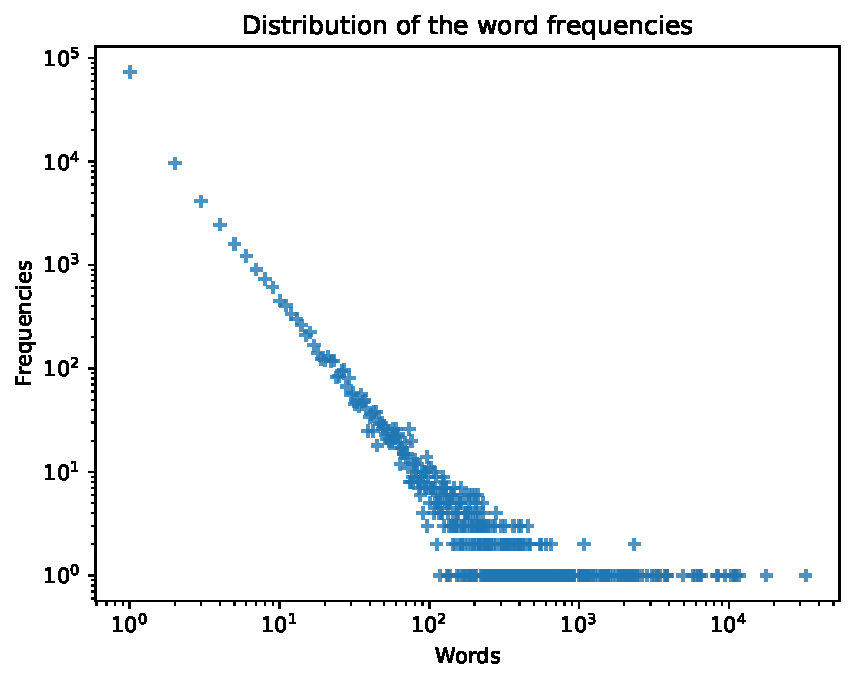
\includegraphics[width=\linewidth]{../images/word_frequencies.pdf}
            \caption{Word Frequencies Distribution.}
            \label{fig:word_frequencies}
        \end{figure}

        \noindent
        As we can see in Figure \ref{fig:word_frequencies}, the words' frequencies follow the well known
        Zipf's law, with a small number of words that appears frenquently, the so called stop words, and the
        majority of the remaining words that appears less and less frenquently. Following the analysis
        proposed in \cite{twitter_as_a_corpus}, I updated the tokens obtained by the early stage of the
        analysis by adding the tags from the application of a Part of Speech Tagging procedure, and I
        observed the tags' distribution between the corpus' documents when considering only the
        positive/negative tweets and the subjective/objective tweets.

        \begin{figure}[h]
            \centering
            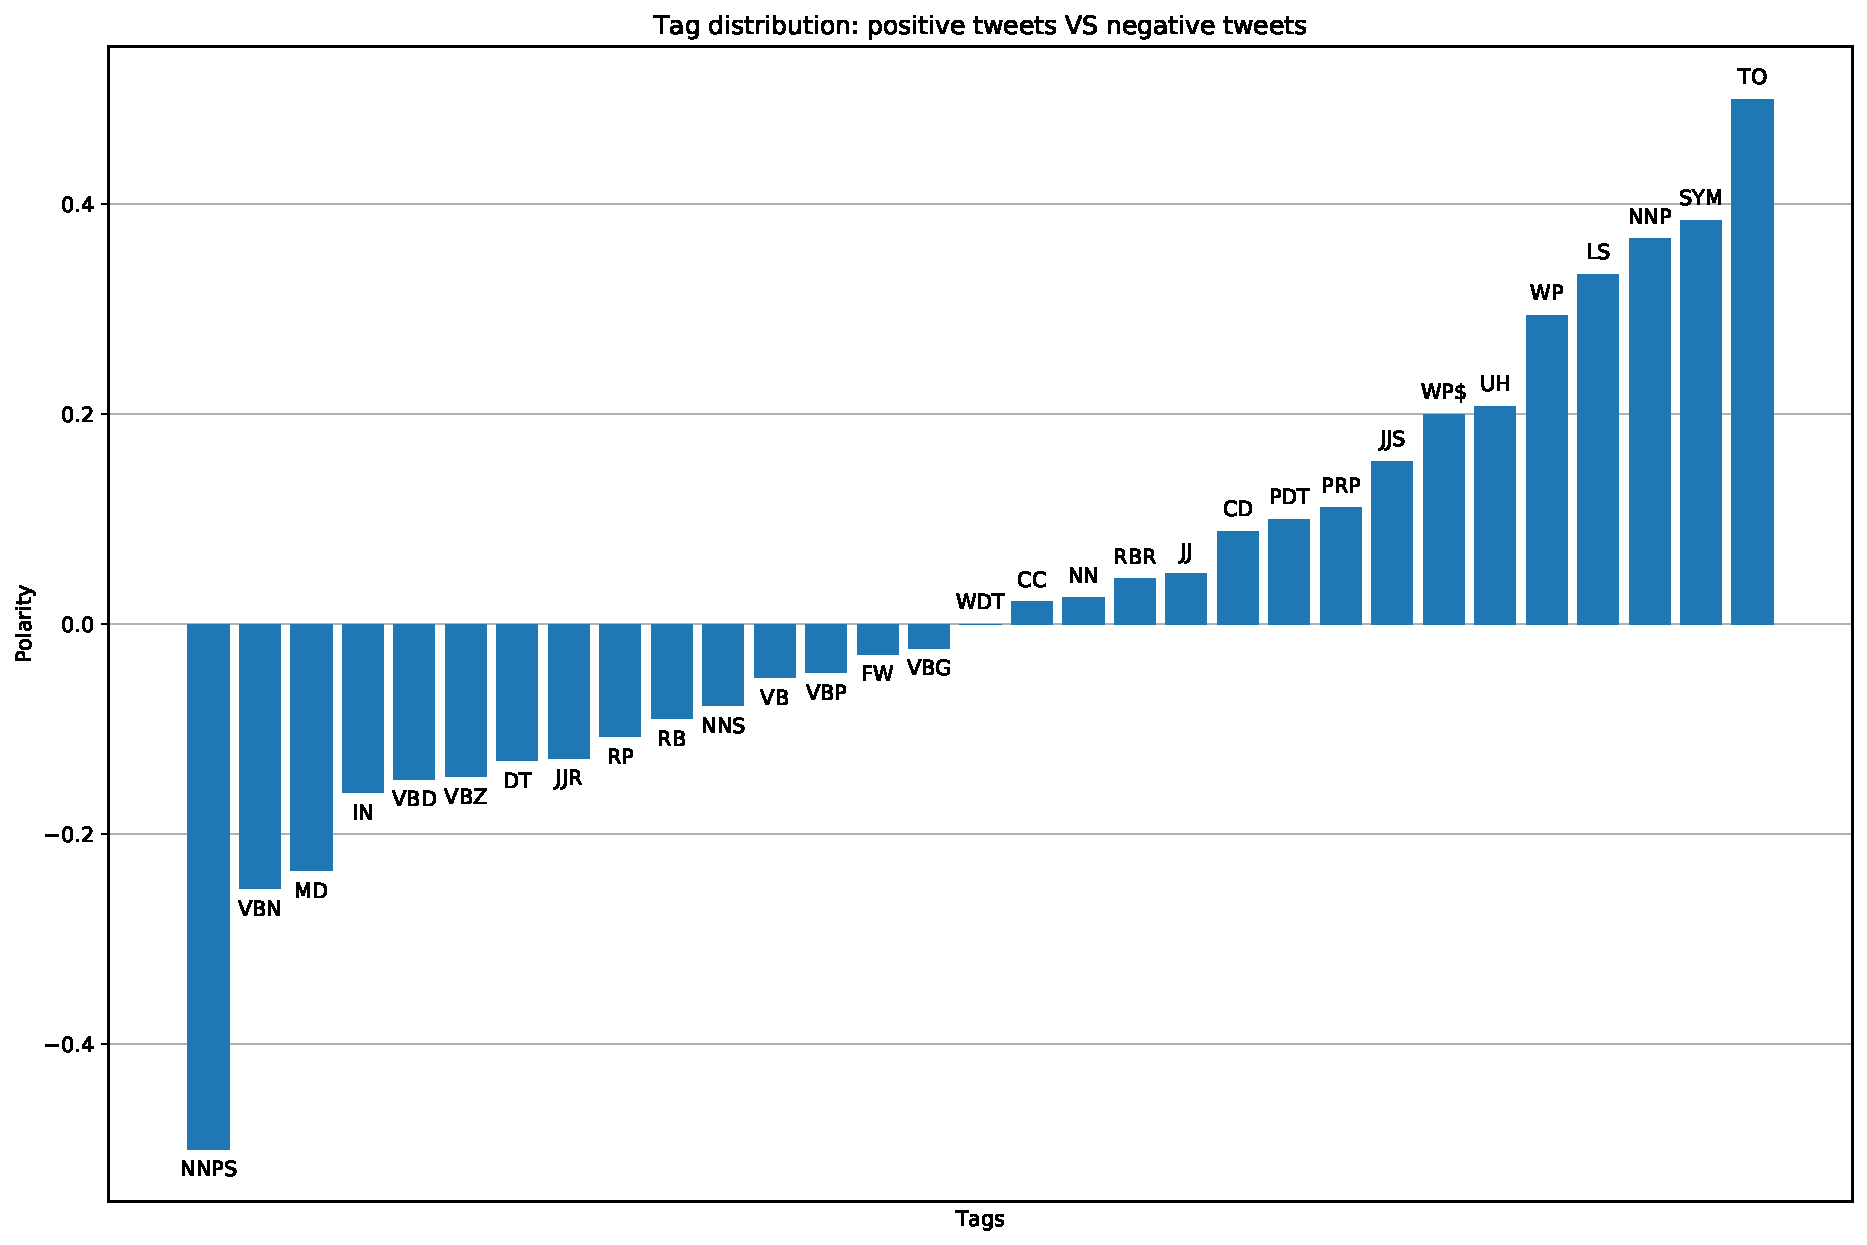
\includegraphics[width=\linewidth]{../images/tag_distribution_positive_vs_negative.pdf}
            \caption{Tag Distribution for Positive and Negative tweets.}
            \label{fig:tags_pos_vs_neg}
        \end{figure}

        \noindent
        As I said before, \cite{twitter_as_a_corpus} proposes the following formula to perform a pairwise
        comparison of tags distributions for each tag and two sets:

        \begin{equation*}
            P_{1, 2}^T = \frac{N_1^T - N_2^T}{N_1^T + N_2^T}
        \end{equation*}

        \noindent
        where $N_1^T$ and $N_2^T$ are numbers of tag $T$ occurrences in the first and second sets respectively.
        As we can see from Figure \ref{fig:tags_pos_vs_neg}, POS tags for positive and negative tweets are not
        distributed evenly, hence we can infer the sentiment behing a document by looking at its tags. We can
        see that the presence of a plural proper noun (NNPS) is a strong indicator for the positive label as
        well as past participle verbs (VBN) and modal (MD). For the negative label, we can see that 'to' (TO)
        is a strong indicator, as well as symbol (SYM) and singular proper nouns (NNP).

        \begin{figure}[h]
            \centering
            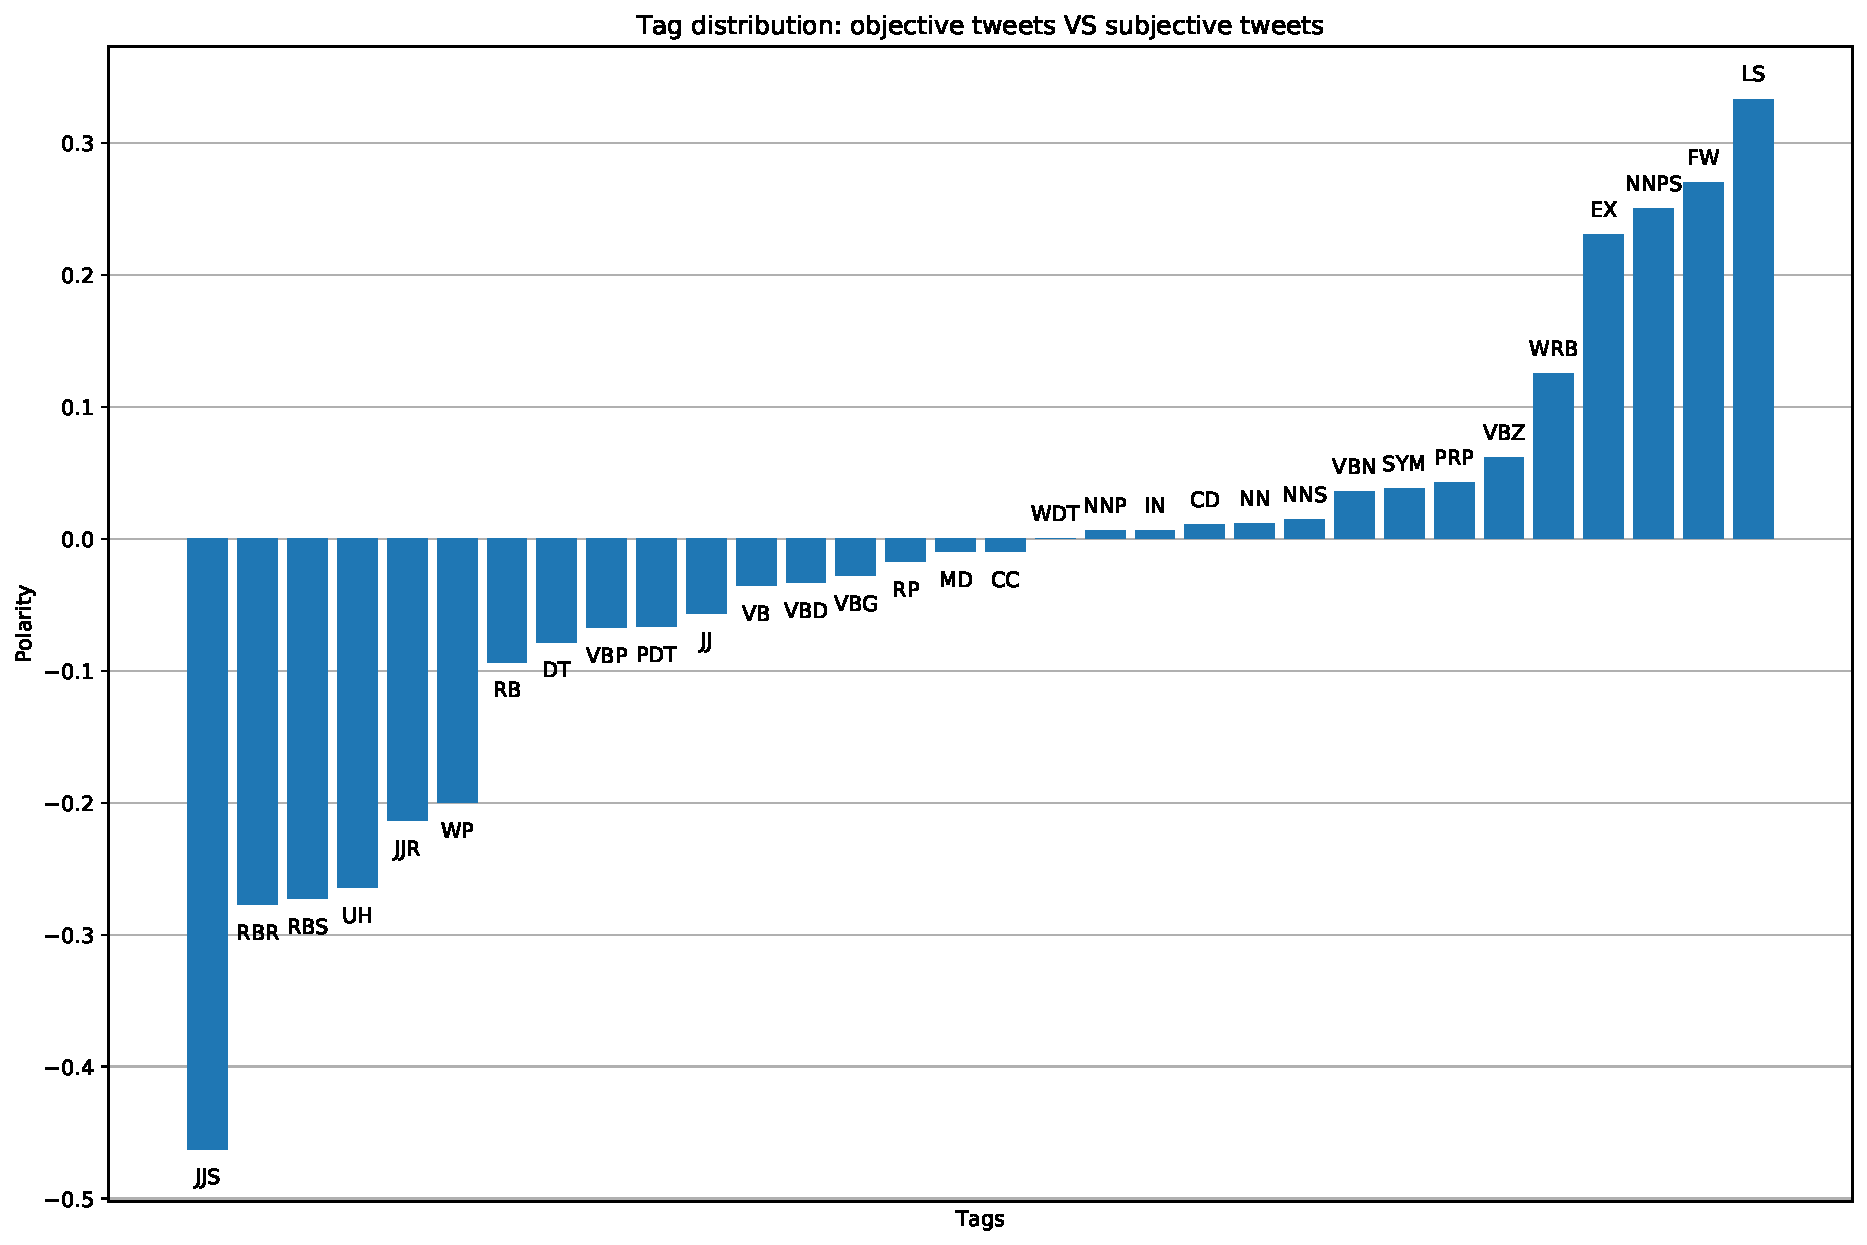
\includegraphics[width=\linewidth]{tag_distribution_objective_vs_subjective.pdf}
            \caption{Tag Distribution for Objective and Subjective tweets.}
            \label{fig:tags_obj_vs_subj}
        \end{figure}

        \noindent
        In Figure \ref{fig:tags_obj_vs_subj} we can observ the tags' distribution for the subjective and
        objective tweets. We can see that possessive wh-pronouns (WP\$), possessive pronouns (PRP\$) and
        superlative adjectives (JJS) are all indicators for objective tweets, while 'to' (TO), foreign words
        (FW) and wh-determiners (WDT) are indicators for subjective tweets. Finally, I have collected some of
        the most used words for positive and negative tweets and represented them via wordclouds, in order to
        provide a better understanding of the sentiments that labels the documents composing the corpus, and for
        providing some visual representation of the informations showed with Figure \ref{fig:tags_pos_vs_neg}
        and Figure \ref{fig:tags_obj_vs_subj}.

        \begin{figure}[h]
            \centering
            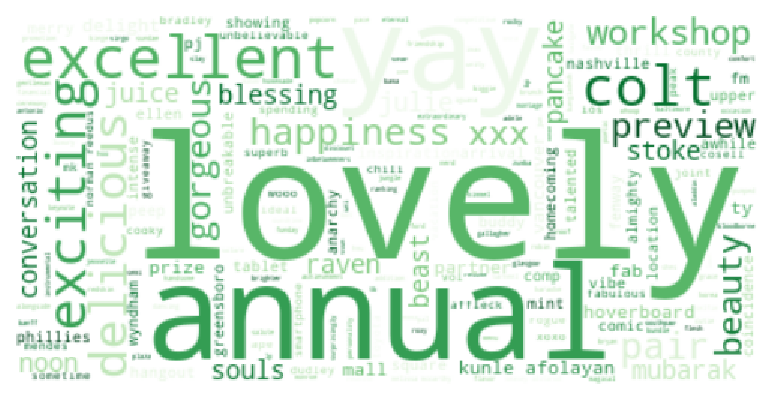
\includegraphics[width=\linewidth]{positive_tokens_wordcloud.pdf}
            \caption{Positive tokens wordcloud.}
            \label{fig:positive_tokens_wordcloud}
        \end{figure}

        \noindent
        In Figure \ref{fig:positive_tokens_wordcloud} we can see the wordcloud for the tokens contained in the
        positive labeled tweets, while in Figure \ref{fig:negative_tokens_wordcloud} we can see the tokens for
        the negative labeled ones.

        \begin{figure}[h]
            \centering
            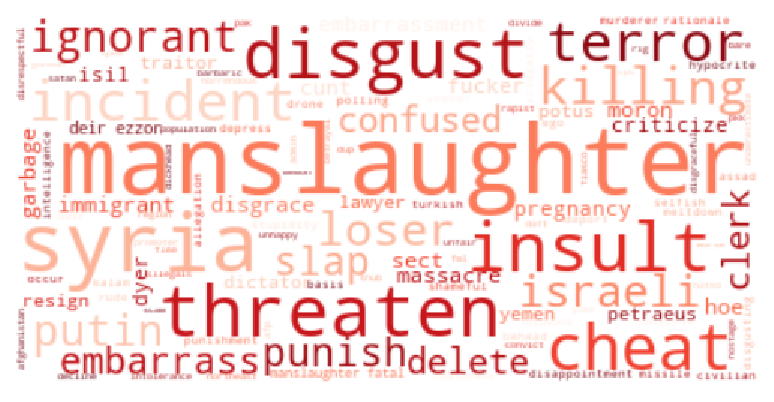
\includegraphics[width=\linewidth]{negative_tokens_wordcloud.pdf}
            \caption{Negative tokens wordcloud}
            \label{fig:negative_tokens_wordcloud}
        \end{figure}
    % section corpus_analysis (end)

    \section{Classification} % (fold)
    \label{sec:classification}
        The Human Language Technologies research's field is very popular at the moment, and, in particular, the
        Sentiment Analysis branch has a rich literature and many tools and resoruces availables for learning.
        Following the results obtained with the analysis reported in Section \ref{sec:corpus_analysis} I have
    % section classification (end)

    \begin{thebibliography}{4}
        \bibitem{twitter_as_a_corpus}
        Pak, Alexander \& Paroubek, Patrick. (2010). Twitter as a Corpus for Sentiment Analysis and Opinion
        Mining. Proceedings of LREC. 10.

        \bibitem{semeval_2014}
        Nakov, P. \& Rosenthal, S. \& Kiritchenko, S. et al. Developing a successful SemEval task in sentiment
        analysis of Twitter and other social media texts. Lang Resources \& Evaluation 50, 35–65 (2016).
        https://doi.org/10.1007/s10579-015-9328-1

        \bibitem{state_of_the_art}
        Mohammad, Saif \& Kiritchenko, Svetlana \& Zhu, Xiaodan. NRC-Canada: Building the State-of-the-Art in
        Sentiment Analysis of Tweets. Second Joint Conference on Lexical and Computational Semantics,
        Volume 2: Proceedings of the Seventh International Workshop on Semantic Evaluation,
        June 2013, Atlanta, Georgia, USA.

        \bibitem{semeval_2016}
        Nakov, Preslav \& Ritter, Alan \& Rosenthal, Sara \& Sebastiani, Fabrizio \& Stoyanov, Veselin.
        SemEval-2016 Task 4: Sentiment Analysis in Twitter. Proceedings of the 10th International Workshop on
        Semantic Evaluation (SemEval-2016), June 2016, San Diego, California.

        \bibitem{esuli}
        Esuli, Andrea. ISTI-CNR at SemEval-2016 Task 4: Quantification on an Ordinal Scale. Proceedings of the
        10th International Workshop on Semantic Evaluation (SemEval-2016), June 2016. Association for
        Computational Linguistics, San Diego, California.

        \bibitem{attardi}
        Attardi, Giuseppe \& Sartiano, Daniele. (2016). UniPI at SemEval-2016 Task 4: Convolutional Neural
        Networks for Sentiment Classification. 220-224. 10.18653/v1/S16-1033.
    \end{thebibliography}
\end{document}
